% First line: specify the class of the document (e.g., article, letter, book, report)
\documentclass{article} 

%=============== Header ===============
%--- Insertion of packages (optional) --- 

\usepackage[pdftex]{graphicx} %package to include pictures 
\usepackage{nicematrix} % for matrix 
\usepackage{amssymb} % package for symbols
\usepackage{amsmath,amsthm} % mathematics mode 
\usepackage{mathtools}
\usepackage{float}           % to plot figures 
\usepackage{url} % to manage urls
 \usepackage{a4} % size 
\usepackage{epsfig} % to manage images
\usepackage[utf8x]{inputenc} 
\usepackage{pgfplots}
\usepackage{apacite} % style of the bibliography 


%=============== Title ===============
\title{Teaching the basics of \LaTeX}
\author{Naomi Chaix \& Alfonso Caiazzo}
%=============== ===============


%=============== Body ===============
\begin{document}
\date{\today} %date 

% Print the title of the document
\maketitle         

% Prints the table of contents
\tableofcontents % write the table of content 


% This starts a new part
\part{}

\section{First section}  %First section 
\subsection{New Subsection}

\subsection{First sub-sections} % First sub-section 
\subsubsection{First sub-sub-sections} %sub-sub section
\paragraph{Introduction} %paragraph 

 LaTeX is a computer language used to format and generate scientific documents. \\
LaTeX is used in particular by mathematicians for the quality of rendering and generation of formulas mathematical.


\section{Layout}

\subsection{Size of the characters} 

\tiny This text is tiny 
\\ % \\ = linebreak (means go to the next line )
\scriptsize This text is scriptsize \\
\footnotesize This text is footnotesize \\
\small This text is small \\
\normalsize This text is normalsize \\
\large This text is large \\
\Large This text is Large \\
\LARGE This text is LARGE \\
\huge This text is huge \\


\subsection{Font size} 

\normalsize % return to normal size 

\textnormal{Normal}   \\ 
\textbf{Bold}   \\ 
\textit{Italic}  \\ 
\textrm{Roman font}  \\ 
\textsf{Sans serif}   \\ 
\texttt{Typewriter}   \\ 
\emph{Emphasize}  \\ 
\textup{Upright}  \\ 
\textsl{Slanted}  \\ 
\textsc{Small Capital }  \\ 
\textmd{Medium serie}   \\ 



\subsection{Alignements} 

% center the text
\begin{center} centred \end{center}     
 
 % put everything on the left
 \begin{flushleft}  aligned to the left \end{flushleft}  
 
% put everything on the right
 \begin{flushright} aligned to the right  \end{flushright}  


\subsection{Verbatim}

Verbatim function restitutes exactly the input text without interpreting any command line nor special characters.  Example: 

\begin{verbatim}
Test with the command \LaTeX  \\ 
and a return to a new line. 
\end{verbatim}


\subsection{Underline}
\underline{Underline}


\section{Underline}

\subsection{Lists}

\begin{itemize}
\item[–] First element
\item[*] With a star
\item[\textbullet] With a point 
\end{itemize}


\section{Mathematics}

\subsection{Equation}

% In order to write an equation, we have to enter the 'equation' environment
\begin{equation} \label{cos2 plus sin2}
\cos^2\theta  + \sin^2\theta = 1
\end{equation}


\begin{equation} \label{easy_eq}
x^2+\int_{\Omega} f(x) \geq 2
\end{equation}
% easy_eq is the 'name' of the equation

% \eqref = creates the reference for an equation
We can reference equations in the text, e.g. \eqref{easy_eq}.
The previous equation in \eqref{cos2 plus sin2}.


\subsection{Specific characters}

We suppose $\epsilon > 0$ an arbitrary threshold :

% The formula is centered and isolated thanks to: \[...\] :
\[
\forall \alpha \geq \epsilon,
f(\alpha) < \frac{1}{2}
\]
Other examples: \\ 
\[
\cos(\theta+\phi)=\cos\theta\cos \phi−\sin\theta\sin\phi
\]

% Thanks to package amssymb:
% Before using a special character, always using $, and end also by $:

%------ Ensembles ------
$
\mathbb{ABC}   \\  % Blackboard Alphanet  
\mathcal{ABC}   \\ % calligraphe Alphabet
\mathfrak{ABC} \\ % Euler Fraktur Alphabet
 $ 
 
$
\overleftarrow{abc} \\
\overrightarrow{abc} \\
\overline{abc} \\
 \underline{abc} \\
\widetilde{abc} \\
 \widehat{abc} \\
\xrightarrow{\text{abc}} \\
\xleftarrow{\text{abc}} \\
 \overbrace{abc}  \\
\underbrace{abc}
$




\section{Pictures}
% To include a picture, you have to use the environment 'figure'

% A figure is a 'floating element' (a float in Latex language), this means
% that Latex will put it where it fits best.
% H = I want the picture here (to be use only if really needed!)
% b = I want it at the bottom
\begin{figure}[htb]
\begin{center}
% includegraphics = include the picture (png, jpeg, pdf, tiff)
% width = specify the width
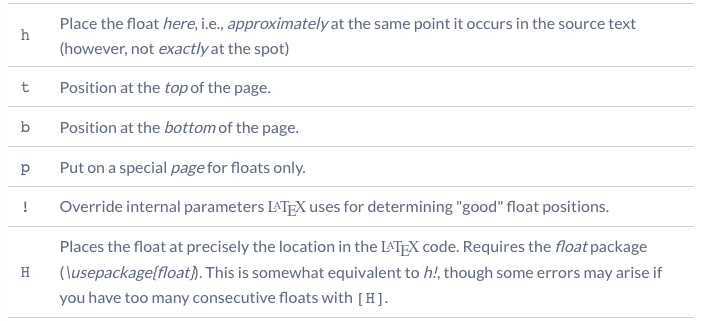
\includegraphics[width=0.75\textwidth]{figures/caption.png}
\end{center}
% This is the caption of the figure
\caption{Label of the pic}
\label{pic} % name of the figure for future references
\end{figure}
We can reference figures in the text, e.g. \ref{pic}

\begin{figure}[H]
\centerline {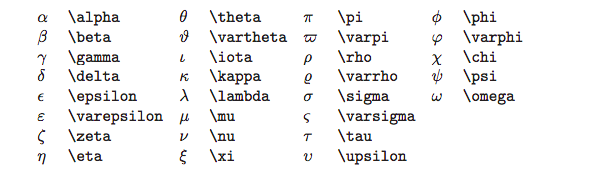
\epsfig { file =figures/grecque.png,width=20cm}}
\caption{Grec symboles}
\label{pic2}
\end{figure}

\begin{figure}[H]
\centerline {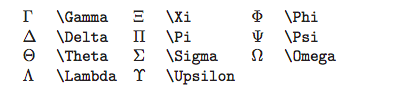
\epsfig { file =figures/grecque2.png,width=15cm}}
\caption{Grec symboles 2}
\label{pic3}
\end{figure}


Here we have a screenshot of how to write the grec symbols, e.g. \ref{pic2}, \ref{pic3}

\section{Additional files}

When compiling a file, with .tex file other ones are produced.

They are a natural byproduct to produce your pdf. The files contain important information. Just keep them.

% Create a list of items with the environment 'itemize'
\begin{itemize}
\item The .log file keeps important information needed for debugging the document.
\item The .aux file keeps track of your labels and citations.
\item The .sync files sync source and pdf-output of the editor/viewer.
\item The .toc file is for a table of contents.
\item The .lof file for a list of figured, .lot file for a list of tables.
\end{itemize}

Important: Keep your working directory clean!



\section{Mention some files from the bibliography}
For citations, first you have to create your bibliography and add a key to each
reference.

% in this case leduc2008road is the key, use \cite to include the citation
Here is the way to refer to some element of the bibliography:  
\cite[Pag 13]{leduc2008road}
Ref to the website:  \cite{ECG}

Creating the bibliography is a separate step, first you link your references to the 
document, then you use bibtex to reference them.

Important (and useful): Your reference list only contains the citations that
you do in the document
%----------------------------------------------------------------------------------------
%	BIBLIOGRAPHY
%----------------------------------------------------------------------------------------

% specify the style of citations 
\bibliographystyle{apacite}
% Here you include your reference database
\bibliography{references/bibli}

%----------------------------------------------------------------------------------------




\end{document}